% todo: wciepać tu więcej dopisów do książek i artykułów naukowych

\chapter{Architektura}

\section{Architektura środowiska i narzędzia}
Na tym stadium pracy bardzo ważne jest dokładne zbadanie wymogów znajdujących się w rozdziale (\ref{chapter:wymagania}), w celu odpowiedniego przygotowania architektury systemu. Błędny wybór, może skutkować ograniczeniami co do zastosowań tego systemu.

\subsection{HomeAssistant -- HA}
Jako system automatyki domowej, kontrolujący wymianę informacji naszego modułu ze światem rzeczywistym wybrano platformę HomeAssistant. Jest to jeden z największych niekomercyjnych systemów tego typu. Jego przewagą w porównaniu do niektórych innych dostępnych na rynku systemów są rzesze fanów i majsterkowiczów, którzy oferują świetne wsparcie i pomagają w rozwiązywaniu problemów. HA skupia się także na prywatności. Programiści open-source jak i użytkownicy systemu zalecają utrzymywanie systemu na swojej własnej infrastrukturze w domu. Dzięki wiernym fanom i samej architekturze projektu system posiada bardzo bogatą bibliotekę integracji z różnymi systemami, od systemów typu Google Assistant w celu dodawania funkcjonalności sterowania głosem, przez własnościowe systemy zarządzania oświetleniem w domu aż po wsparcie dodatkowych bezprzewodowych protokołów komunikacyjnych przeznaczonych do zastosowań domowych. Bardzo ważnym atutem poza szerokim polem różnych integracji jest także system rozszerzeń, gdzie użytkownik może dodać pewną kompletnie nieistniejącą w systemie funkcjonalność do poprawy działania systemu, czy automatyzacji innych rzeczy niezwiązanych z domem.

Na obrazie (\ref{fig:dashboard_example}) znajduje się dostępne na stronie internetowej demo interfejsu mające na celu pokazanie użytkownikom możliwości całego systemu, ale także sposoby komponowania przykładowego panelu zarządzania domem.

\begin{figure}
    \centering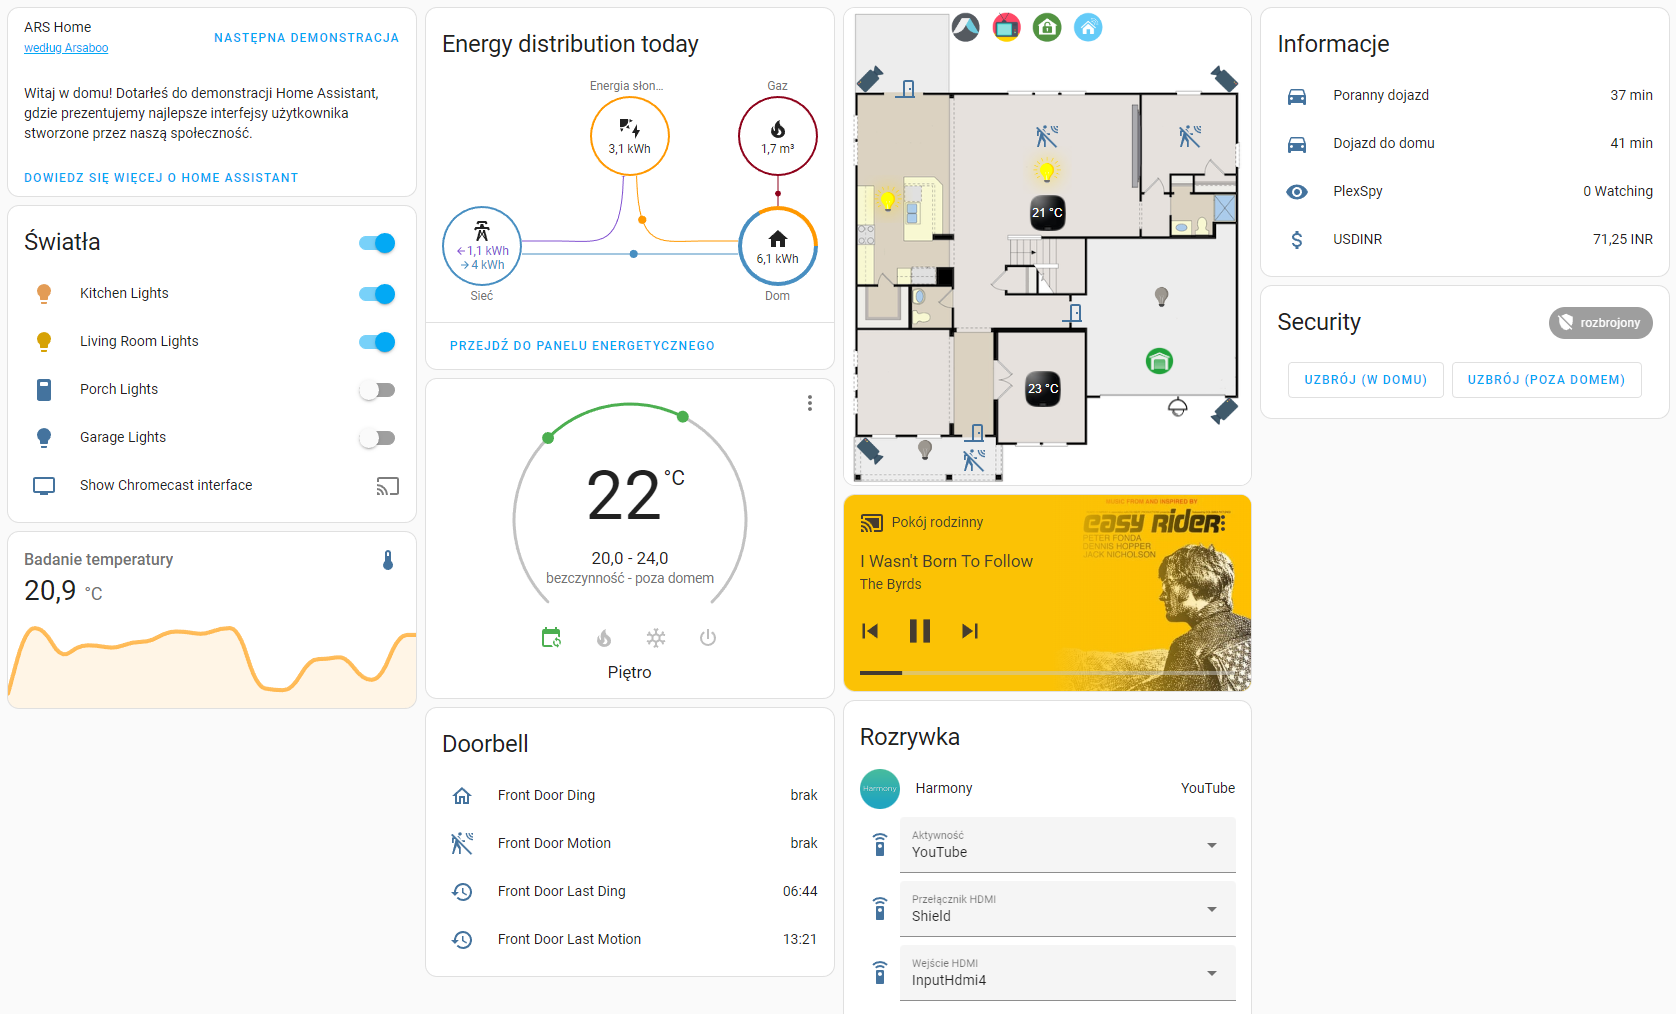
\includegraphics[width=1.00\textwidth]{img/ha_dashboard.png}
    \caption{Przykładowy panel sterowania domem dostarczony przez HomeAssistant} \label{fig:dashboard_example}
\end{figure}

% https://analytics.home-assistant.io/

\subsection{AppDaemon -- AD}
System pozwalający stworzenie modułu samouczącego powinien dawać maksimum możliwości i niezależności, zatem wybrano AppDaemon. AppDaemon to środowisko wykonawczego Pythona, w wielowątkowej architekturze piaskownicy, służące do pisania aplikacji automatyzacji dla projektów automatyki domowej (i nie tylko), których wymogiem jest solidna architektura sterowana zdarzeniami. AD jest od razu gotowe do współpracy z systemem HomeAssistant, co sprawia, że integracja systemów HA/AD jest bezproblemowa. System pozwala natychmiastowo reagować na zmiany stanów urządzeń znajdujących się w domowym środowisku, poprzez korzystanie z asynchronicznej architektury callback.
% Wybór HA jako systemu nadzorczego ogranicza nam pole wyboru rozwiązań które

\subsection{Python i Tensorflow -- tf}
Wykorzystanie struktury HA/AD ogranicza nas do wyboru Pythona jako przewodniego języka programowania w tym przedsięwzięciu. Wybór tego języka nie jest jednak ograniczeniem w tym projekcie, ponieważ posiada on bardzo wielką rzeszę fanów tworzących i udoskonalających paczki kodu dodające nowe możliwości w celu powiększenia pola zastosowań tego języka.

Konkretnym jednym zastosowaniem, który w ostatnim czasie budzi wiele uwagi, jest zastosowanie języka Python do celów uczenia maszynowego. Jedną z bibliotek dostarczających rozwiązania związane z tworzeniem, "uczeniem" i eksploatacją modeli różnego rodzaju sieci neuronowych jest paczka Tensorflow. Tf implementuje wiele gotowych modeli i algorytmów przyspieszających tworzenie modeli sieci neuronowych. Dodatkowo w celu przyspieszenia procesu liczenia błedu propagacji, biblioteka korzysta z różnego rodzaju akceleratorów obliczeń, w tym kart graficznych.

\subsection{Docker}
Ze względu na wymóg niezależności od platformy na jakiej będzie znajdować się ten system, zdecydowano o wyborze jako jednej z głównych technologii, systemu Docker w celu zapewnienia aplikacjom pracującym w jego środowisku odpowiednich warunków niezależnie od systemu operacyjnego na jakim się znajdują. Dodatkowym powodem, który sprawił że wybrano tą technologię jest gotowe wsparcie systemów HA i AD do pracy w konteneryzowanym środowisku bez dużej ilości konfiguracji. Gotowe obrazy aplikacji znajdują się w sieci, a ich instalacja pod warunkiem posiadania środowiska Docker jest bardzo prosta i szybka.

Dodatkowo narzędzia które dostarcza Docker, pozwalają na tworzenie własnych kontenerów i udostępnianie ich innym co sprawi, że nie będzie to rozwiązanie przygotowywane specjalnie pod konkretne środowisko automatyki.

\subsection{Pozostałe narzędzia i biblioteki}
W celu zarządzania środowiskiem programistycznym, wykorzystano platformę Pipenv, która to ułatwia zarządzanie wirtualnymi środowiskami języka Python oraz ułatwia instalację wszystkich bibliotek potrzebnych w danej bazie kodu. Aby wytworzyć gotową paczkę kodu która dalej, która zostanie zainstalowana w AD, wykorzystano narzędzie setuptools. Do wszelakich numerycznych obliczeń oraz interfejsu z Tensorflow została wykorzystana biblioteka numpy. Automatyzowanie środowiska programistycznego zostało wykonane za pośrednictwem Makefile. 

W celu poprawy jakości możliwego w przyszłości rozszerzenia projektu, zdecydowano o skorzystaniu z kilku programistycznych udogodnień. Cała praca podczas tworzenia będzie zapisywana w systemie kontroli wersji git, gdzie będzie można cofać lub wprowadzać zmiany w kodzie na różnych gałęziach niezależnie od siebie. Dodatkowo skorzystano z narzędzia pre-commit, dzięki któremu przed każdym zapisem konkretnej wersji modułu do systemu kontroli wersji, na kodzie będzie przeprowadzana statyczna analiza oraz pewne porządki mające na celu poprawę jakości pracy nad kodem.


\subsection{Podsumowanie}
Na obrazie (\ref{fig:architektura}) znajduje się zaproponowana architektura wysokopoziomowa środowiska. Urządzenia automatyki znajdujące się w  domowym środowisku będą komunikowały się z HomeAssistant w celu aktualizowania swojego stanu, ten będzie przesyłany dalej do AppDaemon gdzie będzie znajdował się nasz moduł obsługujący wybrane zdarzenia. Korzystając z informacji o zdarzeniu, system będzie przewidywał następną akcję i wykonywał pozostałą przewidzianą w danym epizodzie zmianę stanu. Informację o poleceniu zmiany stanu będzie obsługiwał AD, który to dalej bedzie przesyłał tą informację do HA, który zdecyduje jak z danym urządzeniem się skomunikować i jaką wiadomość wysłać. 

\begin{figure}
    \centering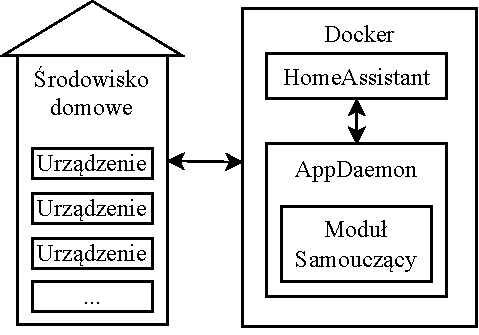
\includegraphics[width=.45\textwidth]{img/architecture.pdf}
    \caption{Proponowane środowisko rozwiązania problemu.} \label{fig:architektura}
\end{figure}

Wewnątrz bloku z modułem samouczącym znajdzie się dopiero kod napisany w języku Python, który będzie reagował na zmiany stanu i w odpowiedni sposób go preparował do przekazania modelowi sieci neuronowych a następnie przekształcany do formy umożliwiającej sterowanie urządzeniami w domu.

\section{Architektura modułu}
Ze względu na wymóg obsługi różnych typów urządzeń oraz źródeł danych, bardzo ważnym aspektem do zaprojektowania jest struktura systemu tłumaczącego dane na takie które, zrozumie biblioteka Tensorflow, zaprojektowanie samych modeli głębokich sieci neuronowych, ale także tłumaczenie wygenerowanej przez model odpowiedzi do takiej, którą zinterpretuje reszta modułu.

\subsection{Dane wejściowe i wyjściowe}
System zarządzania automatyką domową podczas swojej pracy zbiera informacje na temat zmian stanów urządzeń którymi steruje i zapisuje je w lokalnej bazie danych. Nie jest ona jednak dostępna w łatwy sposób dla programisty. AppDaemon w swoim interfejsie programistycznym udostępnia możliwość ściągnięcia historii zmian wybranego urządzenia z ostatniego czasu. Dane przekazane z zapytania do aplikacji są w postaci listy słowników języka Python o strukturze zawartej w listingu (\ref{listing:appdaemon_history}), z listowania usunięto wszystkie nieważne dla modułu pola. Słownik to pewna struktura danych w której informacja jest zawarta w wartościach dla konkretnego klucza \cite{book:learning_python}.

\begin{listing}
\begin{minted}{python}
[
    {
        "entity_id": "input_boolean.test_switch_1",
        "state": "off",
        "last_changed": "2023-09-11T13:07:52.856406+00:00",
        "last_updated": "2023-09-11T13:07:52.856406+00:00"
    },
    ...
]
\end{minted}
\caption{Historyczne informacje na temat stanu urządzenia pochodzące z systemu AppDaemon.} \label{listing:appdaemon_history}
\end{listing}

Warto zauważyć, że informacja zawarta w polu \verb+state+, ma inne znaczenie w zależności od typu urządzenia czy źródła. W przypadku urządzenia typu przerzutnik stabilny o binarnych pozycjach, dane w kluczach \verb+state+ oraz \verb+last_changed+ wskazuje na czas kiedy zaszła zmiana do jakiego stanu, a w przepadu zwykłego przycisku, wystarcza samo pole ze stanem, ponieważ znajduje się tam czas ostatniej zmiany. Wartości pola stanu nie ograniczają się do prostych wartości, system HomeAssistant dodaje kilka dodatkowych wirtualnych urządzeń, które zmieniają swój stan raz dziennie, a ich wartość stanu przy każdej zmianie przyjmuje czas, np. następnego wschodu czy zachodu słońca.

W celu zaspokojenia wymagania integracji z wieloma urządzeniami system powinien na podstawie dostarczonej mu informacji o typie urządzenia tłumaczyć ciąg historycznych zmian na dane treningowe do modelu sieci. Aby rozszerzenie tego rozwiązania było możliwe przez użytkownika, proponuje się, aby system korzystał z klas abstrakcyjnych. Pozwoli to na stworzenie bazowego obiektu i funkcji jakie powinno obsługiwać dane urządzenie w celu współpracy z modułem \cite{book:czysty_kod}. Dodatkowo wymusi to na użytkowniku tworzącym dodatkowe elementy, stworzenie wszystkich wymaganych funkcji, a nie jej pewnej części, co pomaga w redukcji błędów programistycznych.

W celu odpowiedniego przygotowania danych wyjściowych pochodzących z sieci neuronowej, można skorzystać z zaproponowanego wyżej kodu obsługującego dane wejściowe poprzez stworzenie dodatkowych funkcji obsługujących przemiane danych. % , które muszą zostać stworzeone do prawidłowego działania systemu.

Proponowana struktura danych na której moduł będzie się opierał to zestaw dwóch macierzy (\ref{eq:opis_stanu}). Pierwsza zawierająca informacje o aktualnym stanie systemu składająca się z $u$ informacji wejściowych nazywana macierzą stanu, druga składająca się z $w$ skalarów opisująca zmiany w stanach nazywana macierzą przejścia. 

\begin{align}
    \begin{split}
        \mathbf{S}_t = \left[s_1, s_2, \dots, s_u\right] \\
        \mathbf{Z}_t = \left[z_1, z_2, \dots, z_w\right]
    \end{split}
    \label{eq:opis_stanu}
\end{align}

% todo: nie mam nigdzie napisane co to epizod, wypadało by tutaj
% &\text{Przykładowo}\ \left[0, 32, 16, 1\right]
% &\text{Przykładowo}\ \left[-1, 0, 0,  1\right]
% Przykładowo zakładając macierz 

Pierwsza z nich opisuje stan środowiska domowego w danym momencie $t$, druga z nich wskazuje na zmianę stanu urządzeń do następnego momentu w czasie $t+1$. Jesteśmy w stanie określić pewną funkcję $G$ w zależności od typów urządzeń i źródeł, która na podstawie aktualnego stanu oraz zmiany w danym momencie, generuje nam następną macierz $\mathbf{S}_{t+1}$ (\ref{eq:opis_przejscia}).

\begin{align}
    G\left(\mathbf{S}_t, \mathbf{Z}_t\right) &= \mathbf{S}_{t+1} \label{eq:opis_przejscia} \\
    \mathbf{Z}_k &= P(\mathbf{S}_k) \label{eq:opis_modelu}
\end{align}

Biorąc powyższe pod uwagę, proponowane rozwiązanie powinno na podstawie macierzy stanu $\mathbf{S}$ w momencie $k$ przewidywać następny zestaw ruchów użytkownika, czyli macierz przejścia $\mathbf{Z}$ dla tego samego momentu w czasie (\ref{eq:opis_modelu}).

\subsection{Architektura głębokich sieci neuronowych} \label{subsec:nn}
Sercem pracy całego modułu są modele matematyczne sieci neuronowych. Ze względu na wymóg minimalnej konfiguracji, ich logiczna konfiguracja, powinna być wybrana tak, aby były w stanie nauczyć się epizodów akcji użytkownika bez zbędnej wielkości i skomplikowania. Dodatkowym powodem ograniczenia skomplikowania takich sieci jest zdecydowane wydłużenie procesu uczenia sieci neuronowych dla tych które, zawierają dużo wag \cite{time_complexity_nn}.

Model sieci neuronowej zawarty w takim module będzie pracował z różnymi typami urządzeń wejściowych gdzie dane będą sformatowane w różny sposób, dodatkowo dane wyjściowe będą musiały być interpretowane przez moduł inaczej, w zależności od celu. Tworzenie dużych i skomplikowanych sieci nie zawsze sprawia, że jest ona w stanie lepiej nauczyć się przekazywanych jej danych ze względu na klątwę wymiarowości \cite{curse_of_dimensionality}.

Biorąc powyższe pod uwagę, proponuje się, aby moduł podczas tworzenia początkowych modeli nie tworzył jednej monolitycznej sieci odpowiedzialnej za wszystkie wejścia i wyjścia, a tworzył tyle sieci, ile jest urządzeń do sterowania. Umożliwi to sieciom lepsze dostosowanie sie do urządzeń i natury ich używania kosztem lekko dłuższego czasu uczenia.

Proponowana struktura takich sieci znajduje się w tabeli (\ref{tab:neural_network}). Pierwsza warstwa w tym modelu będzie zależna od ilości urządzeń i źródeł dodatkowych danych, a ostatnia warstwa będzie zawierała jedno wyjście. Taka struktura, będzie agregowała wszystkie wyjścia do jednej formy dostarczanej reszcie komponentów.

\begin{table}
    \centering\caption{Tabela zawierająca listowanie warstw w pojedynczej sieci neuronowej \label{tab:neural_network}}
    \begin{tabular}{|l|l|l|}
        \hline
        Warstwa     & Aktywacja     & Ilość neuronów    \dnl
        0           & \verb+linear+ & Zależna od ilości urządzeń    \nl
        1           & \verb+ReLU+   & 128               \nl
        2           & \verb+ReLU+   & 64                \nl
        3           & \verb+tanh+   & 1                 \nl
    \end{tabular}
\end{table}

\subsection{Eksport i import sieci}
Aby móc zapisać modele sieci neuronowych, wszystkie części systemu mające z nimi styczność muszą wspierać takie działanie. W szczególności dwoma krytycznymi elementami w przypadku tego modułu samouczącego jest biblioteka Tensorflow oraz tworzony przez nas system konwersji danych. Oba te elementy powinny współpracować ze sobą na tyle dynamicznie, aby różne konfiguracje modeli oraz danych wejściowych były poprawnie obsługiwane.

Biblioteka Tensorflow dostarcza swoje metody na zapis i odczyt modeli do pamięci stałej, ale są one ograniczone z kilku powodów. Jednym z nich jest brak możliwości zapisywania struktury i wag do własnego bufora w pamięci czy swojego deskryptora pliku. Sprawia to, że każda osobna zapisana sieć będzie tworzyła jeden osobny plik na dysku, dodatkowo bez możliwości dołączenia własnych danych. Operowanie na dużej ilości urządzeń obsługiwanych przez moduł będzie generowało jeszcze więcej plików, które mogą zostać uporządkowane do postaci jednego, czytanego raz w fazie rozruchu systemu.

W celu eksportu i importu sieci zostanie zaproponowany teoretycznie autorski sposób serializowania i deserializowania danych \cite{book:serialization_deserialization} w którym wszystkie definicje oraz -- równie ważne -- wagi wyuczonych sieci neuronowych zostaną zapisane w odpowiednim formacie do pliku archiwum \verb+.zip+. Zapisanie wszystkich potrzebnych informacji do odtworzenia całej struktury w jednym pliku ułatwi przenoszenie użytkownikowi systemu między komputerami, ale także odstraszy go od ewentualnego ręcznego zmieniania wartości wag w systemie, poprzez zaciemnienie widocznej struktury.

Proponowana architektura plików wewnątrz archiwum dla każdej z sieci osobno będzie składała się z:
\begin{enumerate}
    \item Surowej deklaracji modelu, w której znajdzie się dokładny opis kształtu i wymiarów każdej z warstw potrzebnej do dokładnego jej odtworzenia.
    \item Pliku z zapisanymi wagami każdej warstwy w sieci.
    \item Pliku z informacjami pośrednimi, które nie są krytyczne do działania systemu.
\end{enumerate}

Dodatkowo w celu określenia czy nie doszło do zmiany dostępnych dla systemu urządzeń oraz w celu zapisania innych informacji ogólnych o wszystkich dostępnych w modelu sieciach będzie potrzebny jeden dodatkowy plik znajdujący się katalogu głównym archiwum.

\subsection{Podsumowanie}
Na rysunku (\ref{fig:architektura_modułu}) znajduje się proponowana struktura całego modułu samouczącego. Dane o stanie i zmianach będą przechodziły strumieniem wgłąb systemu. Dalej po obliczonej na podstawie stanu systemu predykcji, system będzie sterował urządzeniami w środowisku domowym.

\begin{figure}
    \centering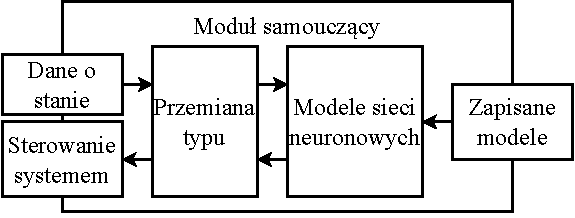
\includegraphics[width=.55\textwidth]{img/architecture_module.pdf}
    \caption{Proponowana struktura działania modułu.} \label{fig:architektura_modułu}
\end{figure}

% \subsection{Sterowanie systemem}

% Sprawia to, że gdy użytkownik posiada istniejącą i skonfigurowaną instalację HomeAssistant z której korzysta, dodanie tego modułu powinno od razu zacząć działać.
% Dane wejściowe obsługiwane przez system przekazywane do biblioteki uczenia maszynowego powinny posiadać swoją pewną strukturę, umożliwiającą Tensorflow pracę.